\chapter{Dynamiczne zwiększanie jakości zdjęć}

Rozwój technologii sztucznej inteligencji (AI) stanowi fundament dla licznych innowacyjnych rozwiązań w dziedzinie przetwarzania obrazów.
Jednym z fascynujących obszarów, gdzie potencjał sztucznej inteligencji jest szczególnie widoczny, jest proces dynamicznego zwiększania jakości zdjęć, nazywany również upscalingiem.
\newline
Upcaling\footnote{\href{https://en.wikipedia.org/wiki/Image\_scaling}{https://en.wikipedia.org/wiki/Image\_scaling}} to technika, która umożliwia zwiększenie rozdzielczości obrazów, co jest niezwykle istotne w kontekście poprawy detali i jakości wizualnej.
\newline
Celem niniejszego projektu jest zastosowanie zaawansowanych algorytmów opartych na sztucznej inteligencji do dynamicznego upscalingu zdjęć.
\newline
Zastosowanie technologii opartej na sztucznej inteligencji pozwala na osiągnięcie znacznie lepszych rezultatów względem tradycyjnych rozwiązań, takich jak interpolacja\footnote{\href{https://pl.wikipedia.org/wiki/Interpolacja\_(grafika\_komputerowa)}{https://pl.wikipedia.org/wiki/Interpolacja\_(grafika\_komputerowa)}}.
\newline
Projekt zakłada udostępnienie serwisu przy użyciu serwisu HTTP, który przyjmuje adres do zdjęcia, a następnie zwraca obraz w poprawionej jakości, oraz zadanej rozdzielczości.
\newline
Przeanalizujemy również już istniejące rozwiązania na rynku.

\chapter{Analiza rynku}

Stosując analizę wyników wyszukiwania popularnych wyszukiwarek (Google, DuckDuckGo, Bing), odnajdujemy wiele powtarzających się rozwiązań.
\newline
Powtarzające się wyniki we wszystkich wymienionych wyszukiwarkach to:
\begin{itemize}
	\item \href{https://www.upscale.media/}{upscale}
	\item \href{https://upscales.ai/}{upscales}
	\item \href{https://www.pixelcut.ai/image-upscaler}{image-upscaler}
	\item \href{https://www.iloveimg.com/upscale-image}{upscale-image}
\end{itemize}

Wszystkie powyższe rozwiązania dostarczają interfejs graficzny, który umożliwia użytkownikowi przesłanie zdjęcia, a następnie otrzymanie obrazu w wyższej jakości.
\newline
Wymagają również subskrypcji, w celu uzyskania dostępu do lepszej jakości, lub możliwości przetwarzania większej ilości zdjęć.
\begin{itemize}
	\item \href{https://www.upscale.media/pricing}{https://www.upscale.media/pricing}
\end{itemize}
\begin{figure}
	\center
	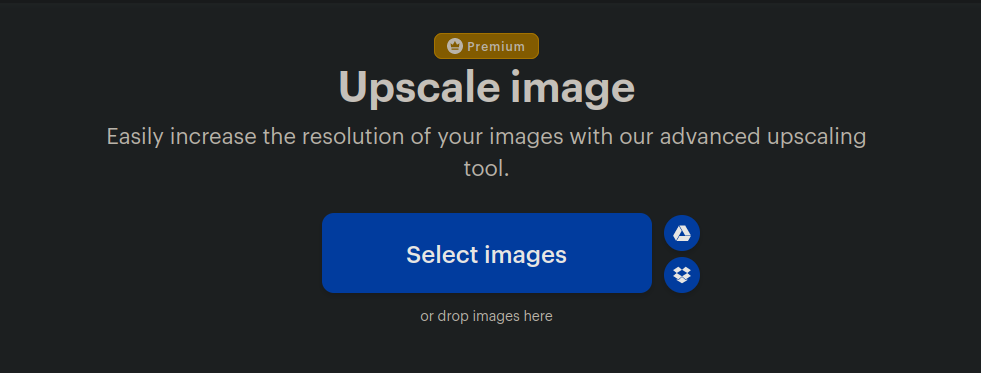
\includegraphics[width=13.0cm, height=3.0cm]{figures/upscale}
	\caption{Interfejs użytkownika serwisu upscale-image}
	\href{https://www.iloveimg.com/upscale-image}{https://www.iloveimg.com/upscale-image}
\end{figure}

\chapter{Analiza zapotrzebowania}

Bazując na formie użycia obrazów na serwisach internetowych, wymagane jest rozwiązanie, które umożliwi dynamiczne zwiększanie jakości obrazów, bez konieczności manualnej interakcji dewelopera z serwisem do zwiększenia jakości zdjęć.
\newline
Aby to osiągnąć, zostanie zaimplementowany serwis, który udostępnia interfejs HTTP, przyjmujący adres zdjęcia, które ma zostać przetworzone, oraz parametry, określające rozdzielczość wynikową.
\newline
Pozwali to na łatwą migrację istniejących serwisów, oraz bezobsługowe działanie.

\chapter{Założenia teoretyczne}

\section{Zasada działania}

Interfejs serwisu do zwiększania jakości zdjęć, powinien akceptować adres zdjęcia, oraz rozdzielczość wynikową.
\newline
Gdy strona internetowa wyświetla obraz, który ma zostać wyświetlony w przeglądarce internetowej, do kodu HTML strony internetowej dodany jest atrybut {\it src}
\newline
\begin{verbatim}
	<img src="https://ftp.pl/images/1.jpg" />
\end{verbatim}

Wskazuje on na obraz znajdujący się na serwerze \textit{ftp.pl}, pod adresem \textit{https://ftp.pl/images/1.jpg}.
\newline
Zakładając, że serwis jest dostępny pod adresem \textit{htttp://serwis.org/}, a zdjęcie, które ma zostać przetworzone znajduje się pod adresem \textit{https://ftp.pl/images/1.jpg}, to adres zwracający obraz w rozdzielczości \textit{1920x1080} to
\newline
\begin{verbatim}
	http://serwis.org/api/1920x1080/ftp.pl/images/1.jpg
\end{verbatim}

\clearpage
\section{Ścieżka działania}

\begin{table}[!h]
    \centering
    \begin{tabular}{p{0.25\linewidth} | p{0.7\linewidth}}
        \hline
        \textbf{Krok} & \textbf{Opis} \\
		\hline
		Załadowanie strony &
		Przeglądarka internetowa pobiera stronę internetową, razem z znacznikami wskazującymi na adresy obrazów. \\
		\hline
		Żądanie HTTP &
		Przeglądarka internetowa po załadowaniu strony internetowej, wysyła żądanie HTTP do serwera, w celu pobrania obrazu. \\
		\hline
		Parsowanie adresu &
		Aplikacja serwerowa parsuje adres, w celu odczytania adresu obrazu, oraz rozdzielczości, w której ma zostać zwrócony obraz. \\
		\hline
		Weryfikacja uprawnień &
		Aplikacja serwerowa weryfikuje po nagłówkach żądania HTTP, czy zostało ono wysłane z strony internetowej, która ma dostęp do serwisu, oraz czy obraz znajduje się na liście zaufanych serwerów. \\
		\hline
		Odpytanie pamięci podręcznej &
		Aplikacja serwerowa sprawdza, czy żądany obraz, w żądanej rozdzielczości został już przetworzony i znajduje się w pamięci podręcznej.
		Jeśli tak, to aplikacja serwerowa zwraca obraz i kończy działanie. \\
		\hline
		Pobranie obrazu &
		Aplikacja serwerowa pobiera obraz z serwera, pod adresem wskazanym w żądaniu HTTP.
		Jeśli obraz nie istnieje, to aplikacja odpowiada kodem statusu HTTP 404. \\
		\hline
		Przetworzenie obrazu &
		Aplikacja serwerowa przetwarza obraz \\
		\hline
		Zapisanie obrazu &
		Wynik jest zapisany do pamięci podręcznej, by nie powtarzać operacji przetwarzania obrazu przy ponownym żądaniu. \\
		\hline
		Zwrócenie obrazu &
		Aplikacja serwerowa zwraca obraz w żądanej rozdzielczości, wraz z kodem statusu HTTP 200. \\
		\hline
	\end{tabular}
\end{table}

% ********** Koniec rozdziału **********